\documentclass[10pt, a4paper, twoside]{article}
%\usepackage[a4paper, total={6in, 10in}]{geometry}
\usepackage[english, russian]{babel}
\usepackage[utf8]{inputenc}
\usepackage{lipsum}
\usepackage{blindtext}
\usepackage{multicol}
\usepackage{graphicx}
\usepackage{color}
\usepackage{tabularray}
%\usefont{T2A}{cmss}{1}{1}
\pagestyle{empty}
\definecolor{Silver}{rgb}{0.721,0.721,0.721}
\graphicspath{ {./images/} }


\setlength{\columnsep}{0.3cm}

\topmargin=-1.1in    
\textheight=11in    
\oddsidemargin= -0.4in 
\textwidth=7.3in

\makeatletter


\begin{document}

\begin{center}
 {\large\bf ОТВЕТЫ, УКАЗАНИЯ, РЕШЕНИЯ} 
\medskip\hrule height 1pt
\end{center}

\begin{multicols*}{2}
\noindent «КВАНТ» ДЛЯ МЛАДШИХ ШКОЛЬНИКОВ\newline
\noindent ЗАДАЧИ\newline
\textit{(см. «Квант» №2)}\newline
\textbf{1. }\textit{Указание. } Начинать надо с самого высокого семиклассника, перестановки можно осуществлять по парам (менять местами самого высокого с тем, кто занимает его  «законное» место, и так далее). При каждой такой перестановке условие, сформулированное в задаче, будет сохраняться (докажите).\newline
\textbf{2. }Поскольку мастер Седов не черноволосый (он отвечает черноволосому) и не седой, то он рыжий; кандидат в мастера не рыжий и не черноволосый, стало быть - седой.\newline
\textbf{3. }См. рис.1.\newline
\newline
\textit{Рис. 1}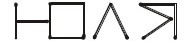
\includegraphics[width=45mm,scale=0.5]{1}\newline
\textbf{4. }5.\newline
\textbf{5. }На чёрных полях вертикальных рядов доски с нечётным номером ставим букву \textit{A}, на остальных чёрных полях ставим букву \textit{B} (рис.2). На белых полях горизонтальных рядов с чётными номерами ставим букву \textit{C}. Число фигур, стоящих на\newline
\textit{Рис. 2}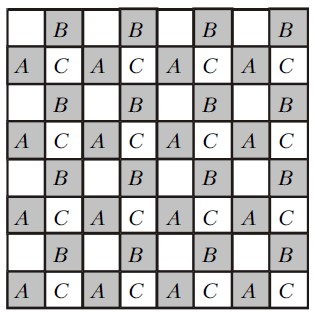
\includegraphics[width=48mm,scale=0.5]{2}\newline
\textit{A}-полях, равно \textit{n}, на \textit{B}-полях - \textit{m}, на \textit{C}-полях - \textit{k}. В силу условия задачи числа \textit{n} + \textit{k} и \textit{m} + \textit{k} являются чётными. Но тогда число \textit{n} + \textit{m} тоже чётное, т.е. на чёрных полях стоит чётное количество фигур.\newline

\noindent РАЗУМНО ИЛИ ЛОГИЧНО?\newline
1) ... читать!   2) ... во всех остальных.\newline
3) ... какая вам разница?  4) ... девятерых попутчиков!\newline
5) ... тех, кто мне не верил!   6) ... Окно!\newline
7) ... станет теплее?   8) ... столько денег!\newline
9) ... найденные.   10) ... железной дороге.\newline
11) ... только два пятьдесят.   12) ... ничего и не делал.\newline
13) ... волос уже нет.   14) ... разбежаться?\newline
15) ... их поносить!   16) ... на твою лошадь.   17) ... хожу.\newline
18) ... врач.   19) ... гостиница слишком низкая.\newline
20) ... с ними разговаривать!\newline
Разделение на «логичные» и «разумные» ответы, конечно, весьма условно. Нормальная разговорная речь практически никогда не бывает совершенно формальной. Даже в такой формализованной системе, как юридический язык, строгий логик нашёл бы много пробелов и не сформулированных явно высказываний. Однако можно заметить, что в задачах 1, 4, 5, 7, 8, 9, 11, 12, 13, 14 правильный ответ использует в основном информацию, данную в самом анекдоте, а в остальных требуется привлечь знания о ситуации.\newline
\newline
\newline
\noindent КОНКУРС «МАТЕМАТИКА 6-8»\newline
\textit{(см. «Квант» №6 за 1997 г.)}\newline
\textbf{11. }Пусть в книге напечатано \textit{C} сказок, причём \textit{n}-я сказка начинается на странице с номером $\textit{H}_\textit{n}$, заканчивается на странице с номером $\textit{К}_\textit{n}$, \textit{n} = 1, 2, ..., \textit{С}. Титул, как известно, всегда располагается в начале книги, а вот аннотация и оглавление могут оказаться как в начале книги, так и в конце. Чтобы не нарушать общности, будем считать, что дополнительной информацией заняты \textit{D} первых страниц, а также 3-\textit{D} страниц в конце книги, где \textit{D} равно либо 1, либо 2, либо 3. Отсюда следует, что $\textit{H}_1$ = \textit{D} + 1, а $\textit{К}_\textit{C}$ = 120 - (3 - \textit{D}) = 117 + \textit{D}. Поскольку каждая сказка начинается с новой страницы, то $\textit{H}_2$ = $\textit{K}_1$ + 1, $\textit{H}_3$ = $\textit{К}_2$ + 1, ..., $\textit{H}_\textit{C}$ = $\textit{К}_\textit{C}-1$ + 1. Сложив последние равенства, получим $\textit{S}_\textit{H}$ - $\textit{H}_1$ = $\textit{S}_\textit{K}$ - $\textit{К}_\textit{C}$ + \textit{C} - 1, где $\textit{S}_\textit{H}$ = $\textit{H}_1$ + $\textit{H}_2$ + ... + $\textit{H}_\textit{C}$ - сумма номеров страниц, на которых сказки заканчиваются. Выражая $\textit{H}_1$ и $\textit{K}_\textit{C}$ через \textit{D}, а также учитывая, что по условтю задачи $\textit{S}_\textit{K}$ = 5$\textit{S}_\textit{H}$, отсюда получаем $\textit{S}_\textit{H}$ = $\frac{117-\textit{C}}{4}$. Число $\textit{S}_\textit{H}$ может быть целым лишь в случае, когда \textit{C} равно 1, 5, 9, 13, ..., т.е. имеет вид \textit{C} = 4\textit{m} + 1, где \textit{m} - целое неотрицательное число.\newline Оценим снизу значение $\textit{S}_\textit{H}$. Так как $\textit{H}_1$ = \textit{D} + 1, $\textit{H}_2 \ge$ \textit{D} + 2, $\textit{H}_3 \ge$ \textit{D} + 3, ..., $\textit{H}_\textit{C} \ge$ \textit{D} + \textit{C}, то\newline
$\textit{S}_\textit{H} \ge$ (\textit{D} + 1) + (\textit{D} + 2) + ... + (\textit{D} + 3) = $\frac{\textit{C}(\textit{C} + 2\textit{D} + 1)}{2} \ge \frac{\textit{C}(\textit{C} + 2\cdot1 + 1)}{2}$ = $\frac{\textit{C}(\textit{C} + 3)}{2}$.\newline
Следовательно, $\frac{117-\textit{C}}{4} \ge \frac{\textit{C}(\textit{C} + 3)}{2}$, откуда 2$\textit{C}^2$ + 7\textit{C} $\le$ 117.\newline
Для указанногго вида \textit{C} решения этого неравенства: \textit{C} = 1 и \textit{C} = 5.
Если \textit{C} = 1, то сказка в книге всего одна. При этом $\textit{S}_\textit{H} \le$ 4 и  $\textit{S}_\textit{K} \ge$ 117, откуда $\textit{S}_\textit{K}$/$\textit{S}_\textit{H}$ > 5, что противоречит условию. В случае \textit{C} = 5 распределение сказок по страницам книги может быть, например, таким:\newline
\begin{tabular}{lllllll}
\textit{номер сказки}                                                                                & 1 & 2 & 3 & 4 & 5   & \textit{сумма:} \\
\textit{\begin{tabular}[c]{@{}l@{}}номер страницы,\\ на которой начинается\\ сказка\end{tabular}}    & 3 & 4 & 5 & 6 & 10  & 28              \\
\textit{\begin{tabular}[c]{@{}l@{}}номер страницы,\\ на которой заканчивается\\ сказка\end{tabular}} & 3 & 4 & 5 & 9 & 119 & 140            
\end{tabular}
Таким образом, в книге напечатано 5 сказок.
\textbf{12. } Обозначим угловые меры дуг окружности, как показано на рисунке 3. Тогда
\begin{center}
\hspace{8in}\angle\textit{DAB} = $\frac{1}{2}(\textit{l}_2 + \textit{s}_2 + \textit{l}_3 + \textit{s}_3 + \textit{l}_4 - \textit{l}_1)$\newline
\angle\textit{BCD} = $\frac{1}{2}(\textit{l}_2 + \textit{s}_1 + \textit{l}_1 + \textit{s}_4 + \textit{l}_4 - \textit{l}_3)$\newline
\qquad\angle\textit{DAB} + \angle\textit{BCD} = $\frac{1}{2}(\textit{s}_1 + \textit{s}_2 + \textit{s}_3 + \textit{s}_4) + \textit{l}_2 + \textit{l}_4 - \frac{1}{2}(\textit{l}_1 + \textit{l}_3)$
\end{center}

Аналогично,\\
\hspace{8in}\angle\textit{ABC} + \angle\textit{CDA} = $\frac{1}{2}(\textit{s}_1 + \textit{s}_2 + \textit{s}_3 + \textit{s}_4) + \textit{l}_1 + \textit{l}_3 - \frac{1}{2}(\textit{l}_2 + \textit{l}_4)$\newline
Поскольку по условию $\textit{l}_1 + \textit{l}_3 =  \textit{l}_2 + \textit{l}_4$, то \angle\textit{DAB} + \angle\textit{BCD} = \angle\textit{ABC} + \angle\textit{CDA}, и следовательно, вокруг четырёхугольника \textit{ABCD} можно описать окружность.
\textbf{13. } Одно из возможных решений показано на рисунке 4.\newline
\textbf{14. } Перепишем уравнение в виде (\textit{a} - 2)(\textit{b} - 2) + (\textit{b} - 2)(\textit{c} - 2) + (\textit{c} - 2)(\textit{a} - 2) = 12.
\end{multicols*}

\end{document}